\subsection{Ansteuerung Motor Ballnachschub}
\label{sec:dc}
Die Ansteuerung des Motors für den Ballnachschub wird in der Gruppe 
PREN-ET entwickelt. (Siehe \ref{sec:pren-et} \nameref{sec:pren-et})
%Daher werden hier nur Anpassungen für das Team 27 betrachtet. 
\begin{figure}[h!]
    \centering
    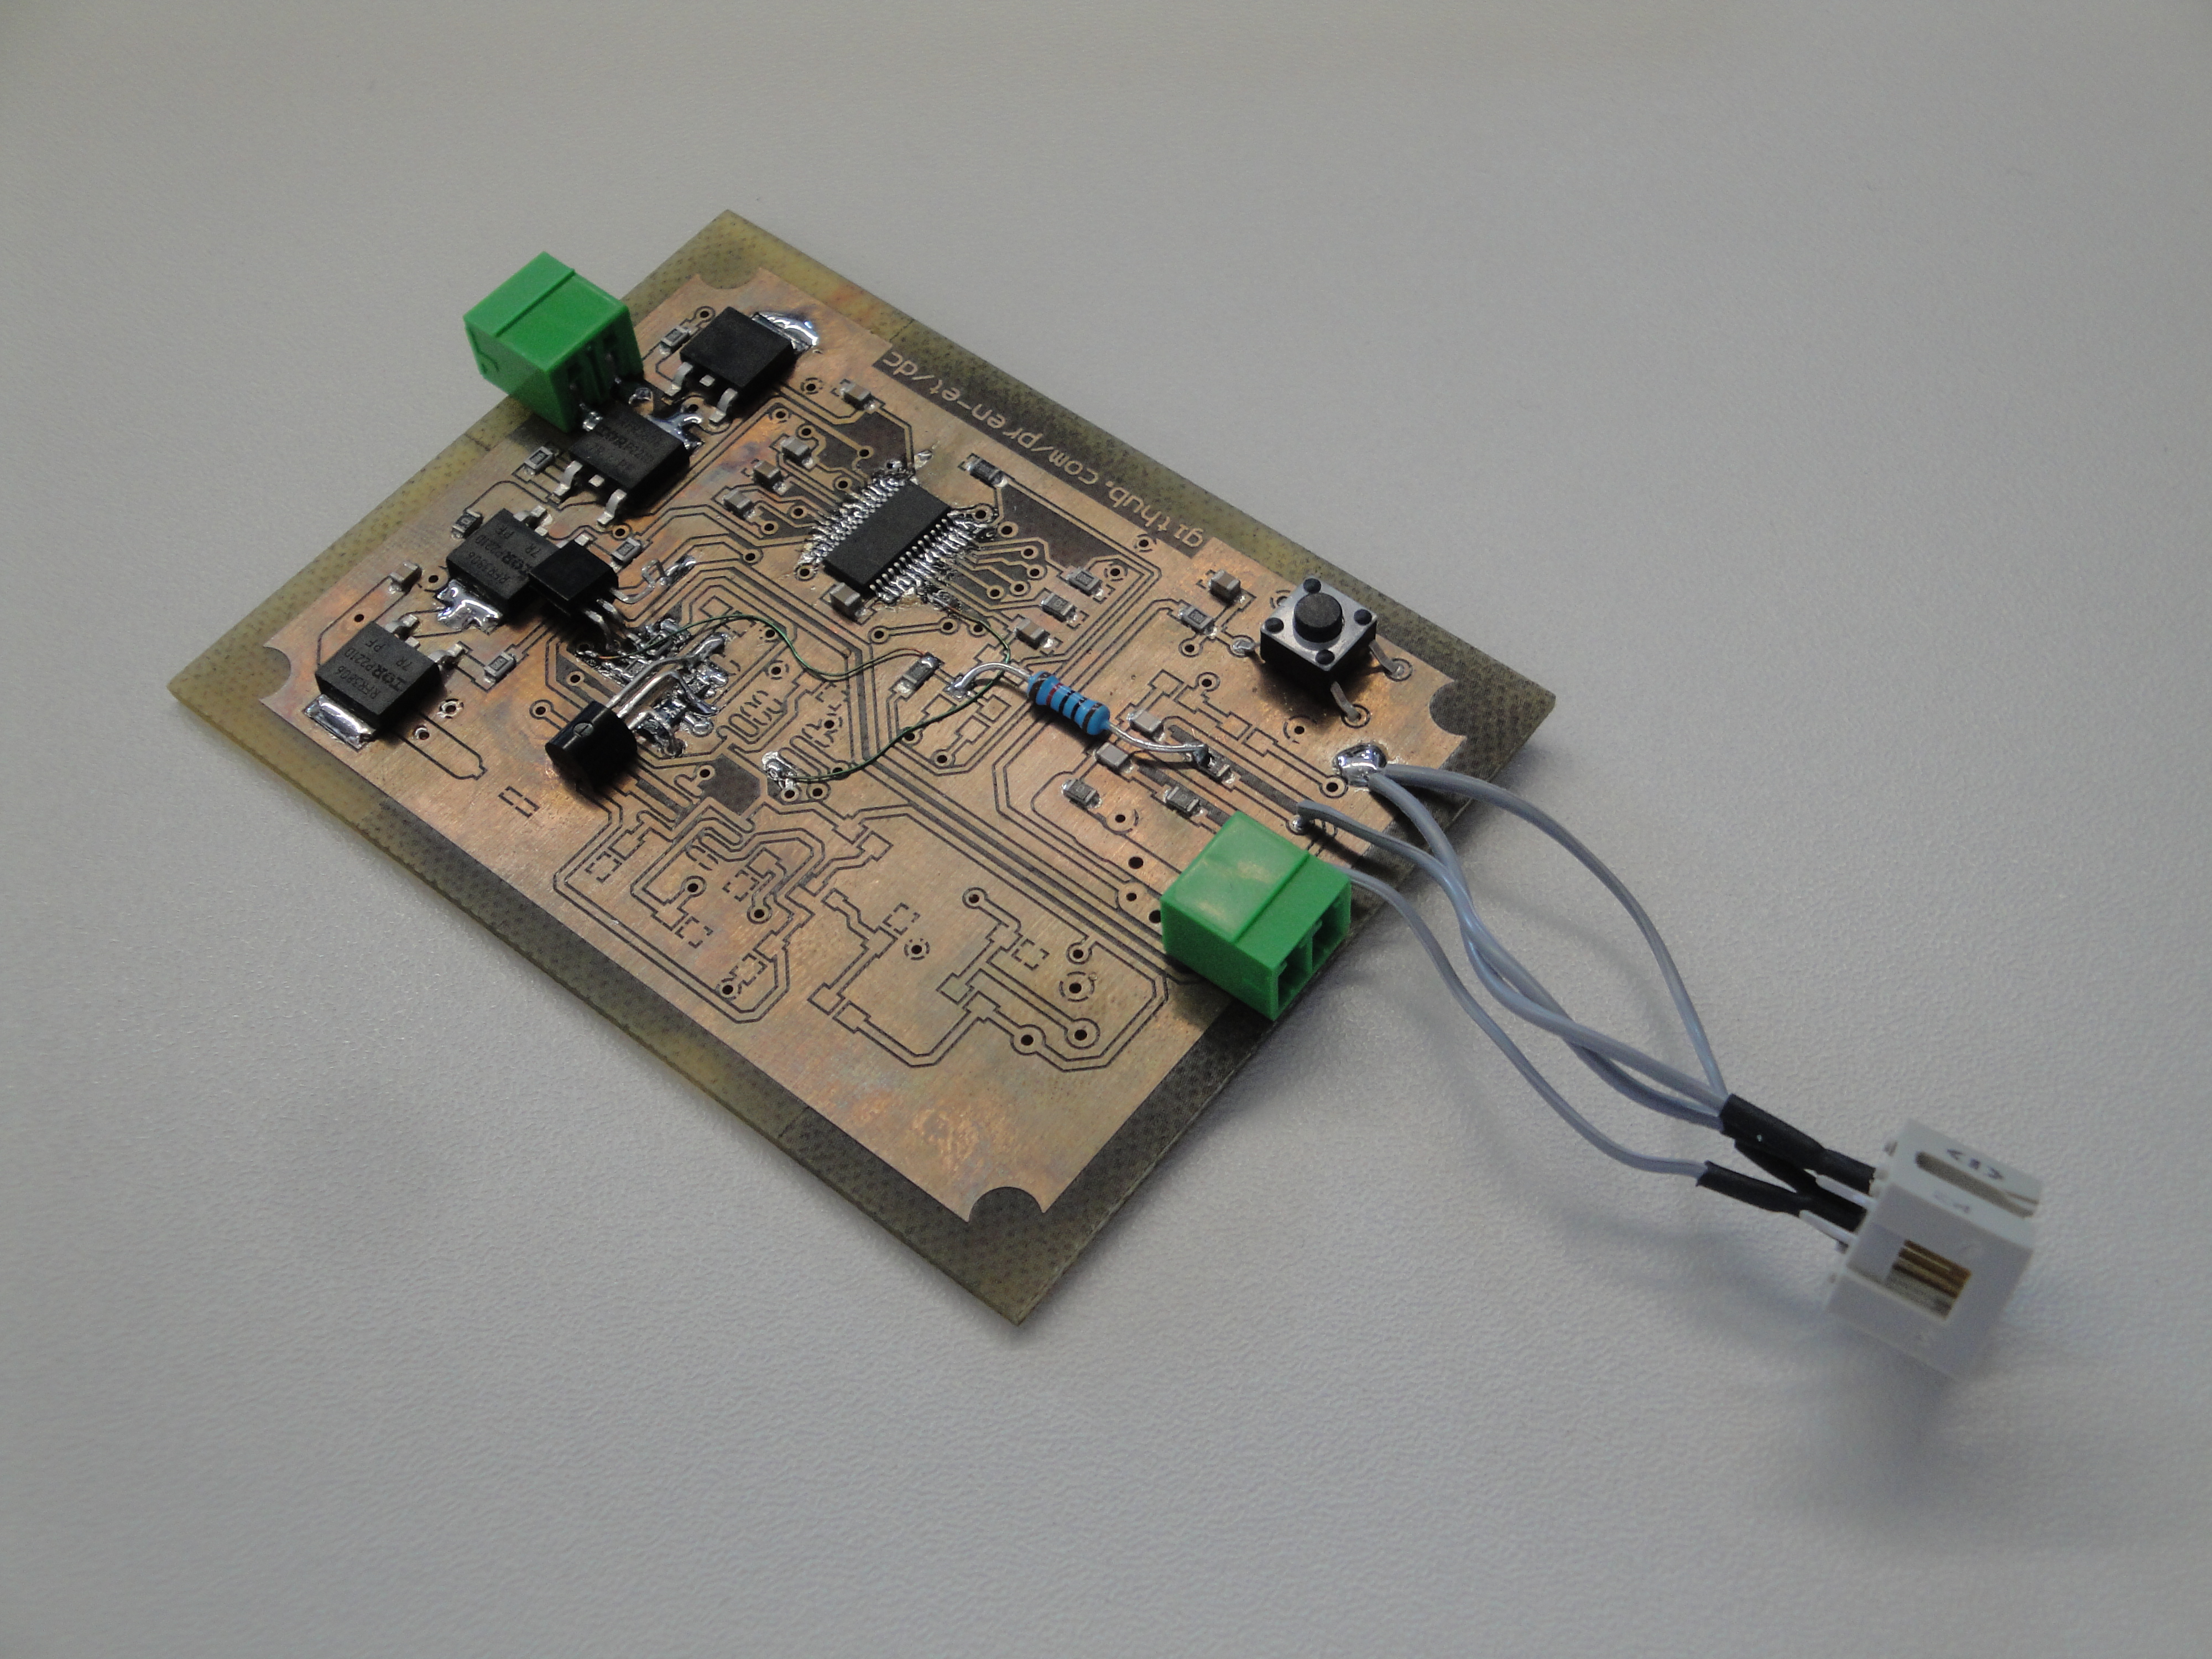
\includegraphics[width=0.7\textwidth]{fig_pcb/DSC02909.JPG}
    \caption{Ansteuerung Ballnachschub}
    \label{fig:dc}
\end{figure}

\noindent
Der Gleichstrommotor für den Ballnachschub wird mit einem 
PWM\footnote{\textbf{P}ulse \textbf{W}idth \textbf{M}odulation} Signal 
angesteuert. Über das Puls-Pausen-Verhältnis kann die Leistung des Motors 
eingestellt werden. Mit dem Signal DIR kann die Drehrichtung des Motors 
gewählt werden. Die interne Generierung des PWM Signals wird nicht verwendet 
und daher nicht bestückt. Da der verwendete Treiber mit Signalspannungen von 
5\si{\volt} arbeitet, werden zwei Pegelwandler, auf dem nicht benötigten Teil 
der Schaltung, diskret aufgebaut. 
